\documentclass[10pt,a4paper]{article}
\usepackage[utf8]{inputenc}
\usepackage[english]{babel}
\usepackage[T1]{fontenc}
\usepackage{amsmath}
\usepackage{amsfonts}
\usepackage{amssymb}
\usepackage{graphicx}
\usepackage{epstopdf}
\usepackage{float}
\usepackage[a4paper,left=3cm,right=3cm,top=2.5cm,bottom=1.5cm]{geometry}
\usepackage[hyperfootnotes=false,hidelinks]{hyperref}
\usepackage{gensymb}
\addtolength{\footnotesep}{3mm}
\usepackage[bottom]{footmisc}

\title{Singing Ferrite}
\author{Kudlankográl GCHD}
\date{}

\makeatletter
\newcommand{\settitle}{\@maketitle}
\makeatother

\begin{document}

\settitle
\thispagestyle{empty}
\addtocounter{page}{-1}


\begin{figure}[H]
\centering
    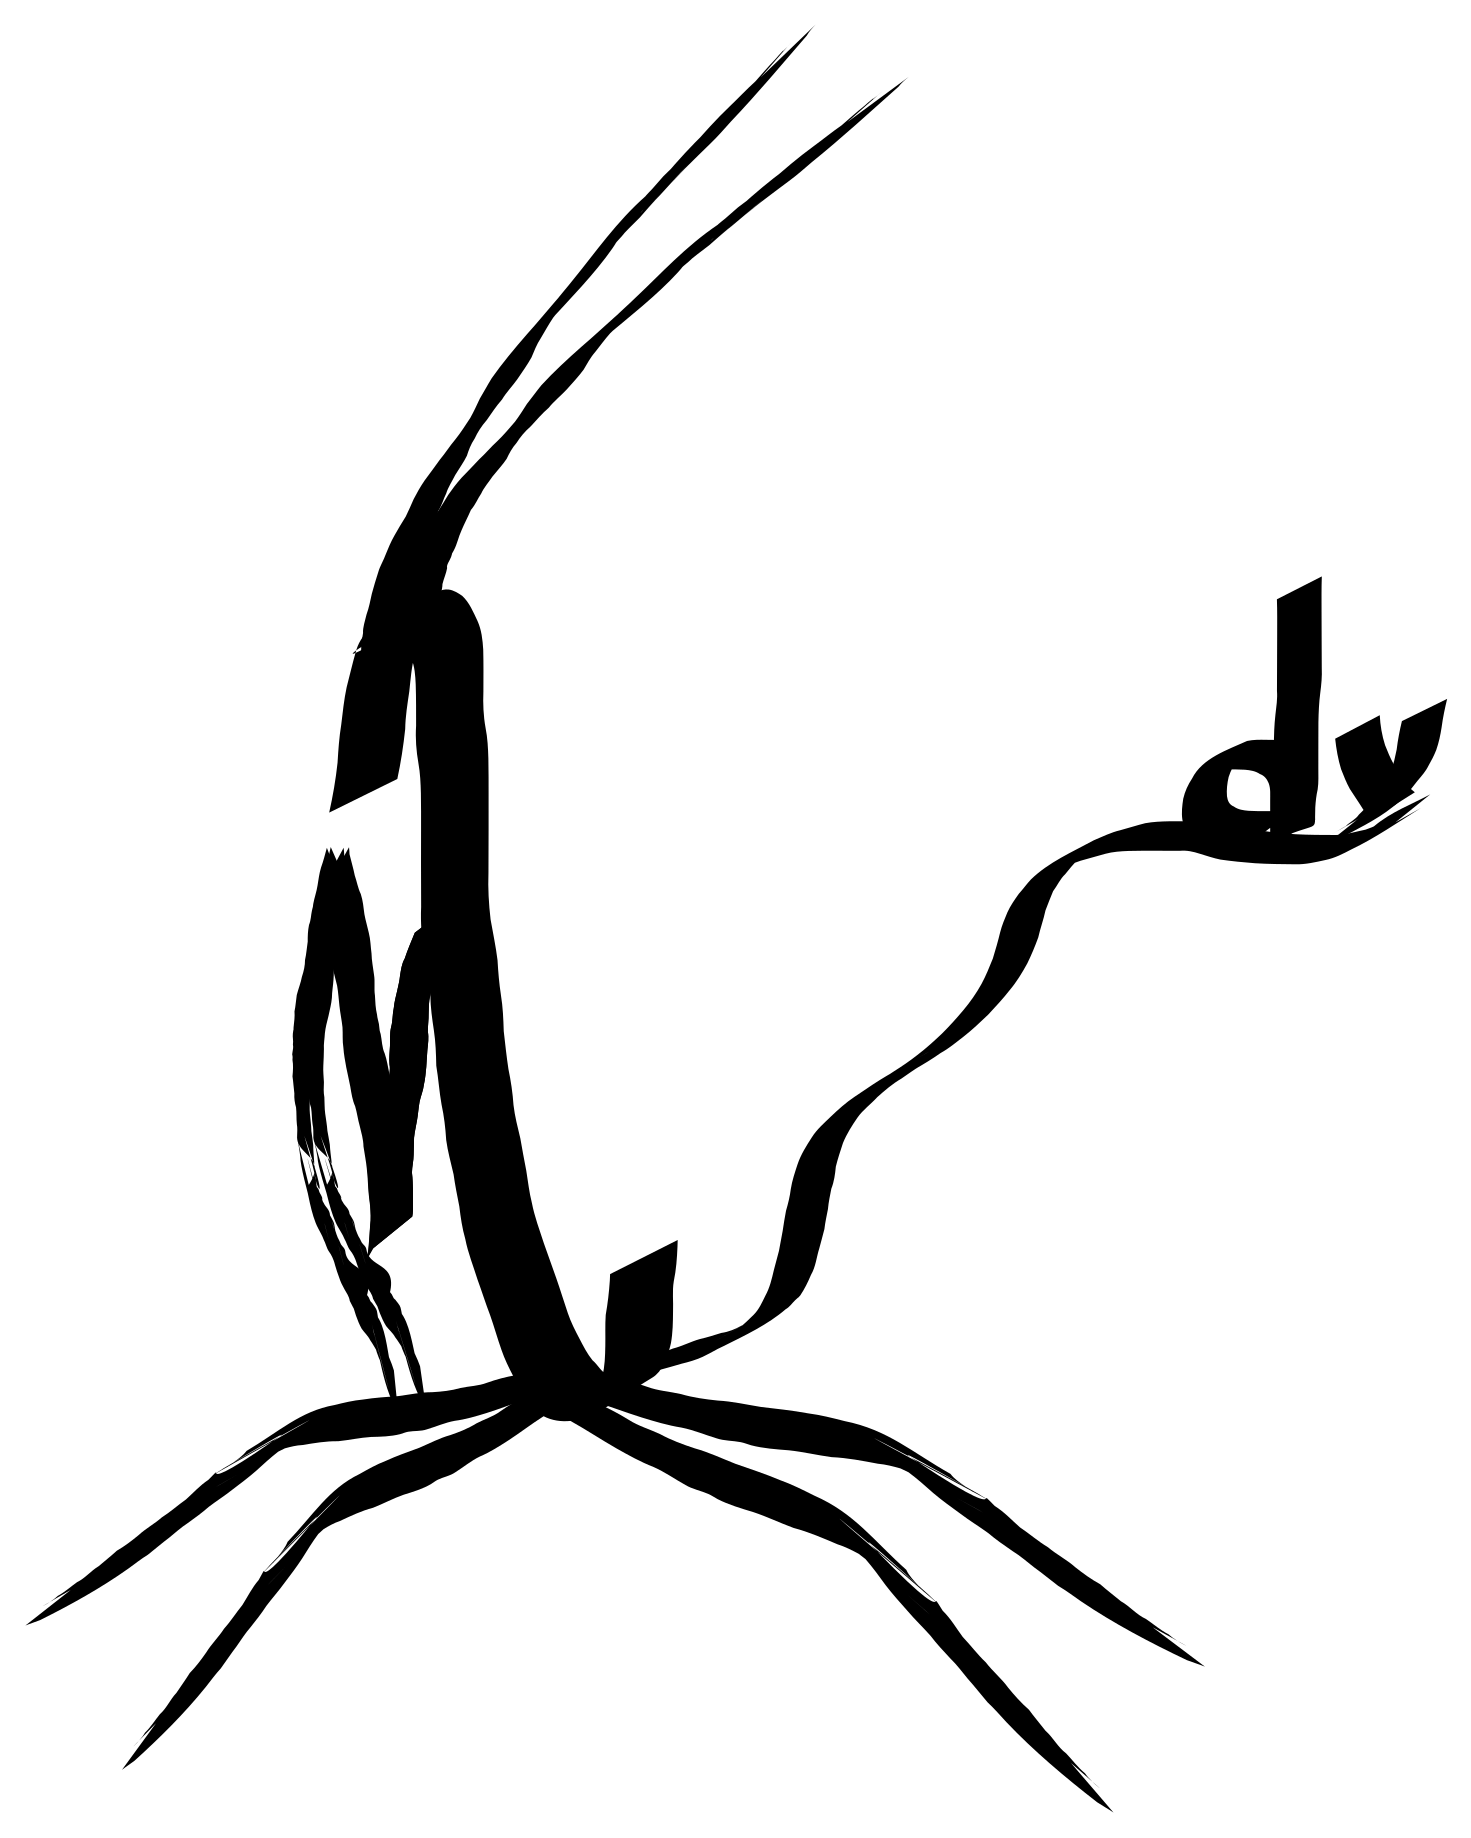
\includegraphics[width=0.95\textwidth]{kudlankogral.png}
\end{figure}

\paragraph{}
Name of the team: Kudlankográl GCHD
\paragraph{}
School: Gymnázium Christiana Dopplera
\paragraph{}
Address: Zborovská 621/45, Praha 5 - Malá Strana, 150 00

\clearpage
\newpage


\author{}
\maketitle
\tableofcontents

\newpage

\section{IYPT 2020 Problem}
Insert a ferrite rod into a coil fed from a signal generator. At some frequencies, the rod begins to produce a sound. Investigate the phenomenon. \footnote{IYPT 2020 Problems | IYPT.org. Official IYPT Website | IYPT.org [online]. Available from: \url{https://www.iypt.org/problems/problems-for-the-33rd-iypt-2020/}}
\section{Abstract}
In this work we tried to study oscillations of ferrite rod caused by changing outer magnetic field. We studied the phenomenon from two points of view: mechanical and electromagnetic. Our mechanical solution was focused on finding natural frequencies of different oscillations in a rod. Electromagnetic solution was mostly an qualitative explanation to some effects we noticed during our experiments. We compared our mechanical theory with experiments and we reached a very good match.
\section{Magnetostrictive hysteresis loop}
In our work we are studying phenomenon which is based on magnetostriction. The magnetostriction is described by a magnetostrictive hysteresis loop showed on picture down here. We used the magnetostriction hysteresis loop described in work named Model of the Magnetostrictive Hysteresis Loop with Local Maximum. Author describes magnetostrictive hysteresis loop and shows, that it is closely related to parabolic curve (Later he describes more concrete model, but for our purpose it’s too complicated).
\footnote{Szewcyk, R.: Model of Magnetostrictive Hysteresis Loop with Local Maximum; Institute of Metrology and Biomedical Engineering, Warsaw University of Technology, 02-525 Warsaw, Poland}


\begin{figure}[H]
\centering
    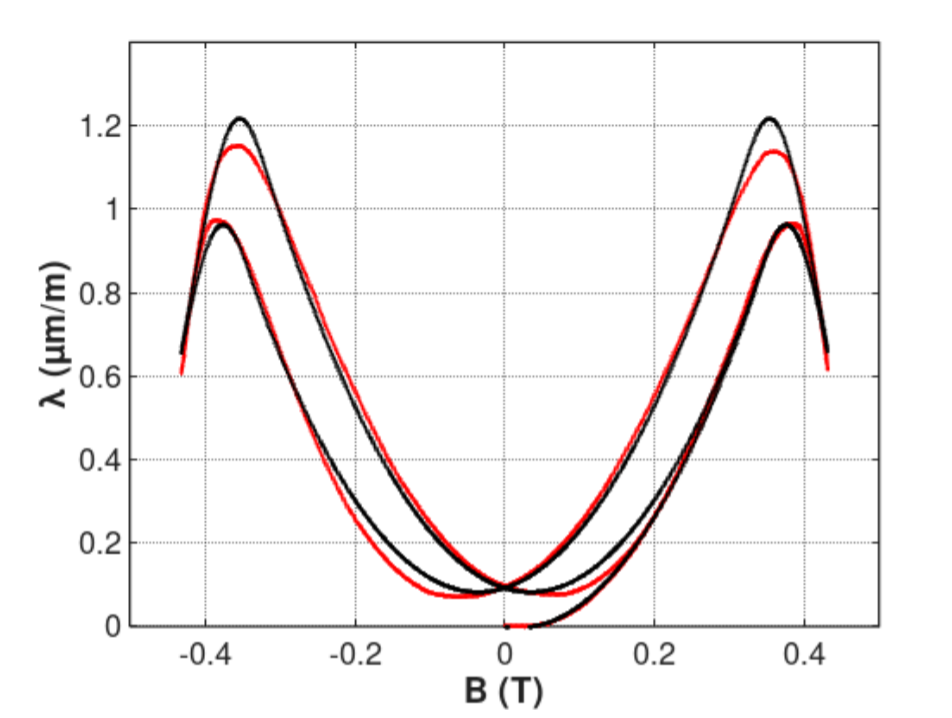
\includegraphics[width=0.7\textwidth]{Magnet.png}
    \label{fig:chart1}
\end{figure}

\newpage
\section{Experiments}
\subsection{Finding magnetostriction effect}
If we change geometry of ferrite rod we change its magnetization. Our very first experiments were focused on finding magnetostriction effect. We inserted ferrite rod into a coil. The coil was connected to oscilloscope. Afterwards we hit the rod with other ferrite (Doesn’t have to  be a ferrite, but we used ferrite). Oscilloscope measured high frequency voltage oscillations in the coil. These were caused by standing wave inside the rod, which changes the magnetization of the whole ferrite rod. We found the magnetostriction effect in our ferrite rod.
\subsection{Trying to produce sound}
Next experiment we did was inserting the ferrite rod into a coil and connecting the coil to a harmonic frequency generator. Our rod was hanging on two strings inside the coil to minimize the friction inhibition effects. We noticed the sound is produced only at some frequencies. For our ferrite rod, which was 15,3 cm long with diameter of 0,8 cm these frequencies were at 1,6 kHz, around 4 kHz, 8,6 kHz, 18,8 kHz, 20,5 kHz. We see, that these frequencies look pretty random.
\subsection{Stationary  magnetic field}
Later we returned to the first experiments, this time with improved setup. We found few interesting effects: if we put a permanent magnet in the vicinity of the ferrite rod , we detect statistically bigger oscillations and a big peak in the beginning. We were interested in this effect so we studied it more deeply. Here we present you few oscilloscope measurements after the hitting the ferrite with another ferrite. First four are oscillations without outer magnetic field, the other four are oscillations with outer magnetic field. We used the experimental setup described in Experiments: Trying to produce sound, with connected oscilloscope.

\begin{figure}[H]
\centering
    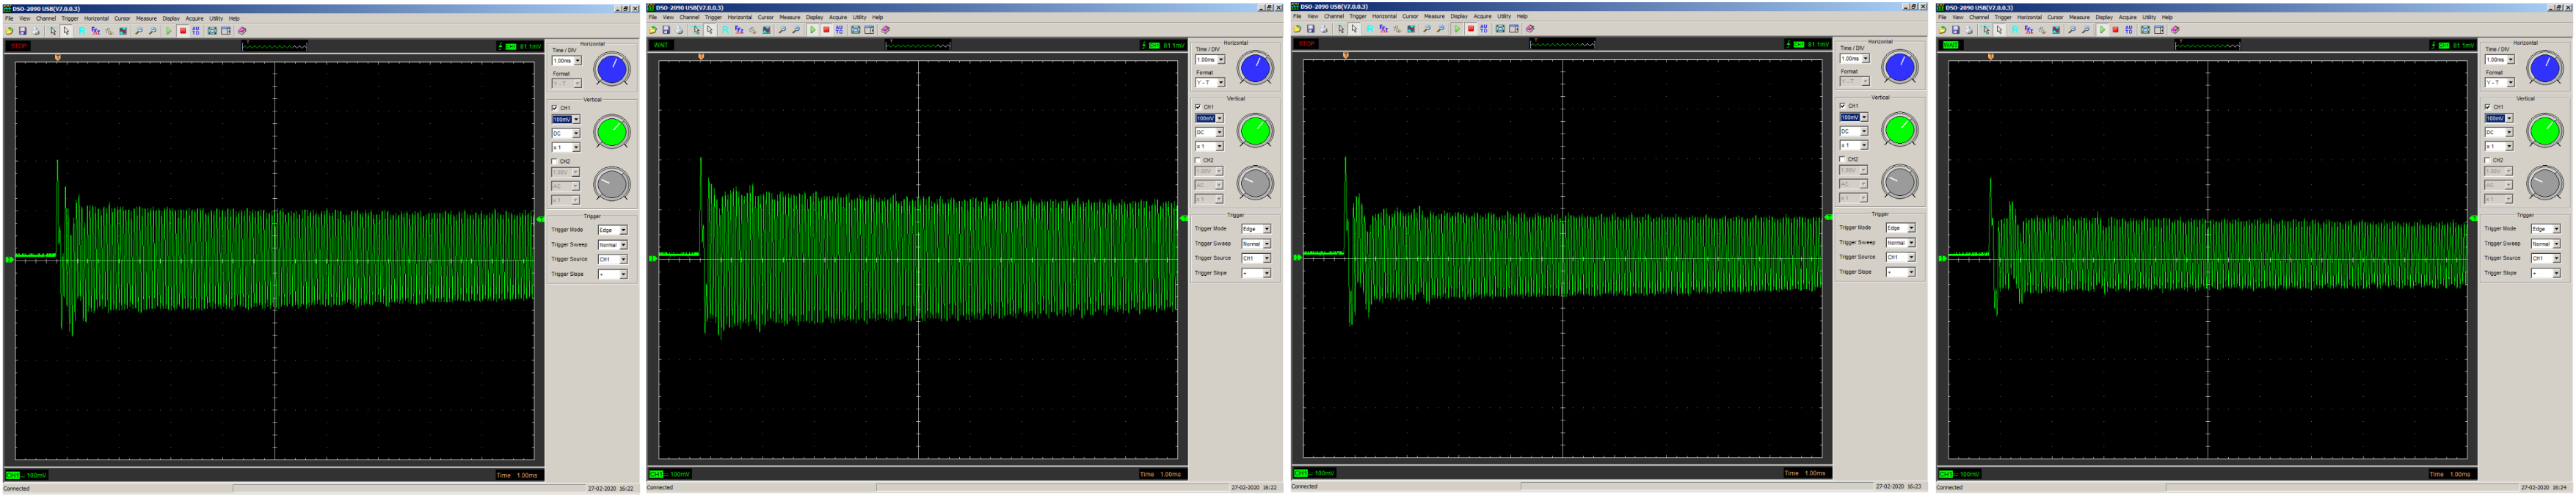
\includegraphics[width=\textwidth]{bezf.png}
    \label{fig:uvod}
    \caption{Voltage in the measuring coil in time without outer magnetic field}
\end{figure}

\begin{figure}[H]
\centering
    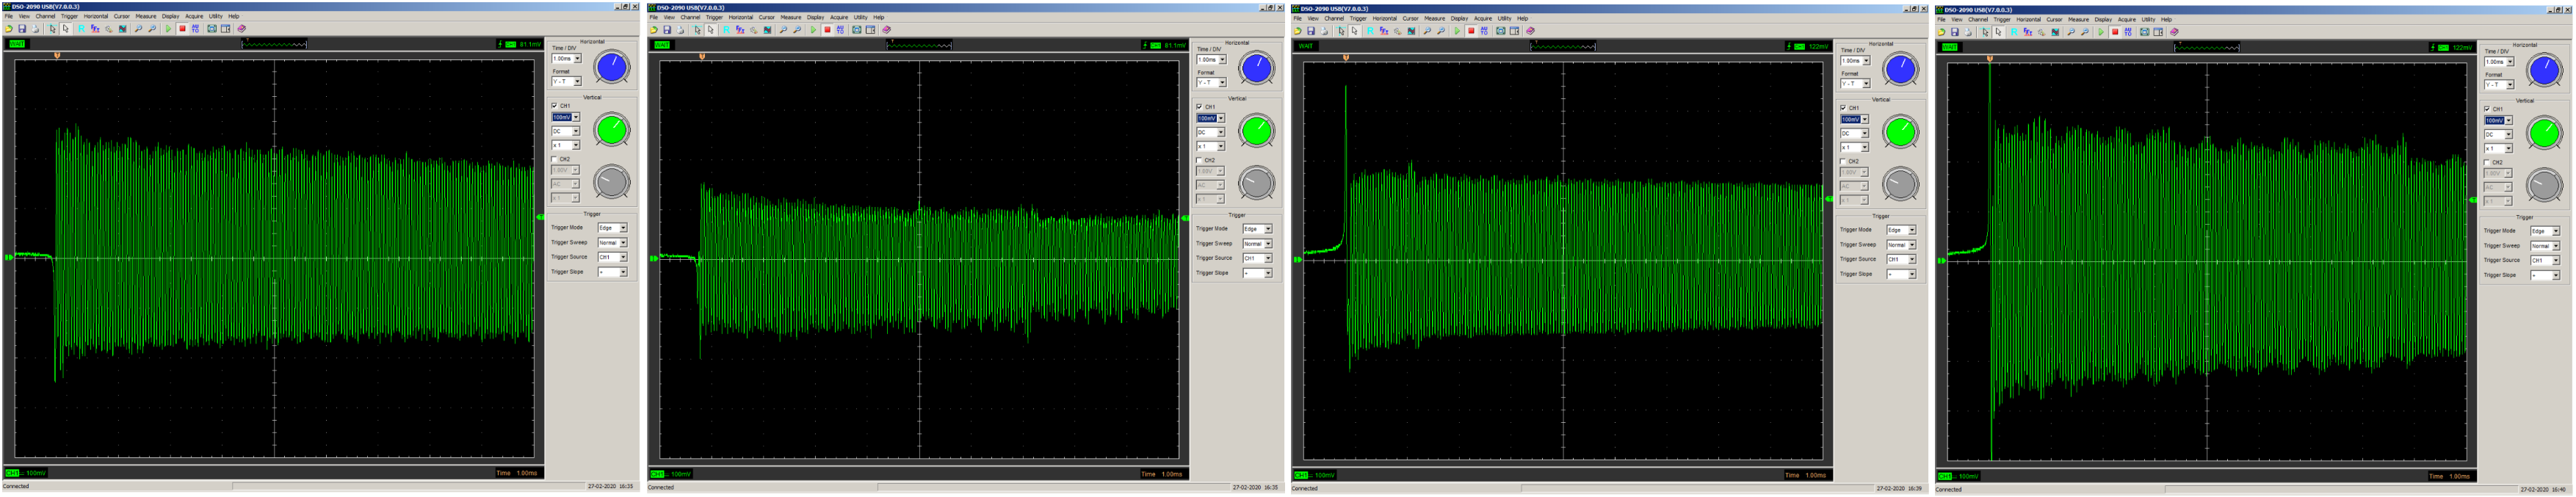
\includegraphics[width=\textwidth]{sf.png}
    \label{fig:uvod}
    \caption{Voltage in the measuring coil in time with outer magnetic field}
\end{figure}

\subsection{Measuring Q-factor}
To ensure that measured oscillations are truly caused by magnetostriction of the ferrite rod we were advised to measure (or calculate based on measurements) Q-factor. If Q-factor is low, then it could mean that these oscillations are not caused by magnetostriction, but by oscillations in measurement circuit. We extracted measured curves to .csv file and then processed the data to find the change of amplitude. At some cases we found an amplitude modulation with frequency around 50 Hz. From the square of the amplitude and from amount of waves we calculated Q-factor of 1,6103. Such a Q factor cannot be produced by the measurement circuit itself, so it must be produced by ferrite. At the picture below you may see analyzing resulting data from oscilloscope.

\begin{figure}[H]
\centering
    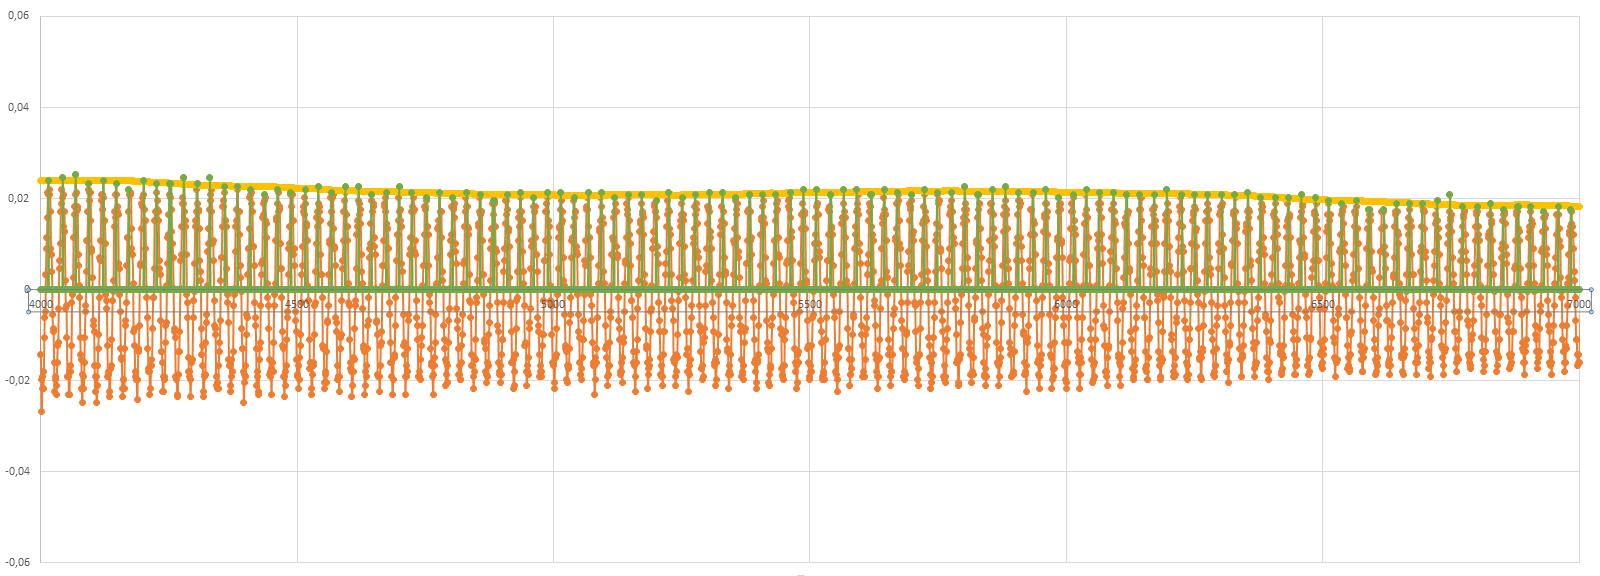
\includegraphics[width=\textwidth]{volt.png}
    \label{fig:uvod}
    \caption{Voltage in measuring coil in time}
\end{figure}

\subsection{Amplitude modulation}
As we mentioned before, one of our experiments showed us an amplitude modulation with frequency around 50 Hz. The effect occurred during experiments with one of our 10cm long rods on the last day of experiments. Because of the 50 Hz frequency we thought, it could be caused by some other magnetic field sometimes occurring in the laboratory. We started to measure the changing magnetic field in the room and we found a changing magnetic field with frequency of 50 Hz and amplitude of 0,001 mT. Sometimes there occurred few signals with higher amplitude. The changing magnetic field was harmonical in one direction in the room, in an orthogonal direction we could not find the harmonical changing magnetic field. The amplitude modulation of the oscillations of ferrite rod were found only sometimes, did not depend on the direction. We conclude these are not caused by the outer magnetic field. We decided to measure acoustic oscillations in the ferrite rod and found the amplitude modulation there as well. You may see the result of measurement of acoustic oscillations on the picture below.

\begin{figure}[H]
\centering
    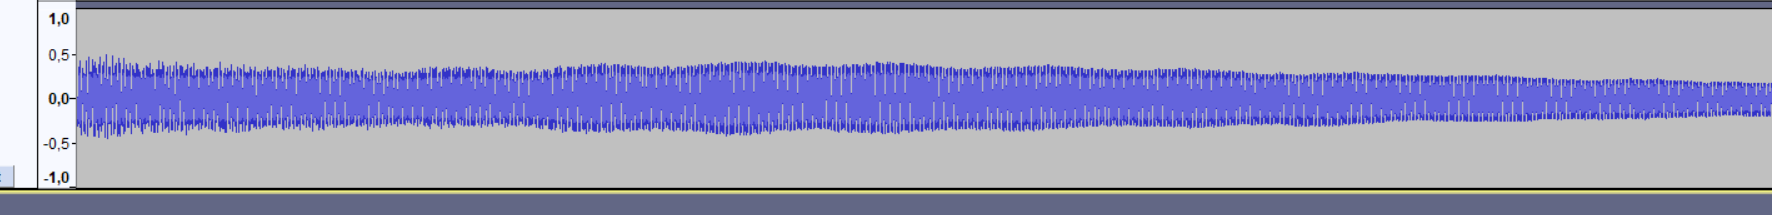
\includegraphics[width=\textwidth]{ampl.png}
    \label{fig:uvod}
    \caption{Measurement of acoustic oscillations}
\end{figure}

We measured another ferrite rod and sometimes found an amplitude modulation of 21 Hz.

\subsection{Powering the coil with measured free rod oscillations}
The final experiment we did was powering coil with amplified signal microphone sensing sound from the ferrite rod. When we did this experiment with 15,3 cm long ferrite rod we detected sound signal around 17,5 kHz. When we did this experiment with 10 cm long ferrite rod we did not detect any sound, but when we put a magnet near the ferrite rod, we started to detect sound around 3,7 kHz.


\newpage
\section{Theory}
\subsection{Experiment n. 1 outcome}
After hitting the ferrite rod we start detecting electrical oscillations in the rod, which means that magnetic flux going through the coil is changing. From that we conclude, that magnetization of ferrite is changing. This can be caused only by magnetostriction effect: After hitting the ferrite rod there appears a standing wave which forces ferrite to change its magnetization.
\subsection{Experiment n. 2 outcome - mechanical solution}
The sound, as we know from experiments n. 2, is produced only at some frequencies. From the knowledge of the magnetostriction and knowledge of general oscillation theories we conclude, that these frequencies are natural frequencies of the ferrite rod. At this point we decided to measure and calculate the natural frequencies of rods made from different materials and with different cut sections geometry. These frequencies can correspond to  either longitudinal, or bending oscillations. To calculate natural frequencies of longitudinal waves in the rod we need to know some material constants and natural frequency shouldn’t depend on the cut section. 
We expect, that the wavelength of the standing longitudinal wave is equal to $\frac{2l}{k}$, where $l$ is length of the rod and $k$ is a natural number. 
From that we know, that $f=\frac{vk}{2l}$, where $v$ is the speed of sound in the ferrite rod. 
From other works we found out, that $v=\sqrt{\frac{E}{\rho}}$, where $E$ is Young's modulus of elasticity and  is density of the material
\footnote{One-dimensional Elastodynamics, available from: \url{http://homepages.engineering.auckland.ac.nz/~pkel015/SolidMechanicsBooks/Part_II/02_1D_Elasticity/02_1D_Elasticity_02_Elastodynamics.pdf}}.
From that we calculated, that lowest natural frequency for our 15,3cm long ferrite rod is around 18kHz (The result can vary depending on the Young's modulus for ferrite: from 14,6Hz to 20,6kHz). But in experiment n. 2 we have measured sound frequencies of 1,6 kHz, 4 kHz and 8,6 kHz, which means the ferrite rod is not oscillating only with longitudinal standing waves. These waves are of some other kind. There is another possibility - transverse standing waves, but, they cannot appear due to the way we are creating the waves inside the material (we are creating longitudinal waves. The only explanation we could think of was a process, when due to some irregularities inside the ferrite rod longitudinal sound waves force ferrite rod to start oscillating with bending standing wave. We decided to calculate the natural frequency of such a bending standing wave. In result we got this expression:
$$f=\frac{2\pi}{\lambda^{2}} \cdot \sqrt{\frac{E}{\rho}} \cdot \sqrt{\frac{I}{S}}$$  \centerline{(Appendix: First mechanical theory)}\\\mbox{}\\
where $\lambda$ is length of bending wave, $I$ is secondary moment of inertia of the ferrite rod cut section and $S$ is area of the ferrite rod cut section. This expression gave us natural frequency for our 15,3 cm long ferrite rod of around 1,5 kHz, which seems close to the measured value 1,6 kHz, as well as for 10 cm long ferrite rod we calculated natural frequency of 3,4 kHz, instead of the measured 3,7 kHz. Conclusion is that in our theory there is an inaccuracy. We were expecting the bending wave to be harmonical, but it is not, otherwise angular momentum is not conservative (from Euler-Bernoulli Beam theory
\footnote{\label{Euler} Parks, D. M.: Euler-Bernoulli Beams: Bending, Buckling and Vibration; Department of Mechanical Engineering MIT}
there would be some moment applied to every piece of rod, which does not appear in our phenomenon). As we didn’t know the shape of the bending standing wave, our next result was having an coefficient $k$ which we could not calculate:
$$f=\frac{k}{l^{2}} \cdot \sqrt{\frac{E}{\rho}} \cdot \sqrt{\frac{I}{S}}$$  
\centerline{(Appendix: Second mechanical theory)}\\\mbox{}\\
where $k$ is some sort of coefficient we could theoretically calculate, if we knew the shape of the bending standing wave, and $l$ is length of the rod.
Fact we did not calculate the coefficient $k$ could seem disturbing, and whole work could seem useless, but important thing about this coefficient is, that it has the same value for any material, length of rod or even any cut section shape. The coefficient is always the same, if the curvature of the rod is same. We measured the coefficient $k$ experimentally (we expected the speed of sound in ferrite to be 5470 m/s):
$$k = 1,77$$
\centerline{Our sinusoidal theory gave us coefficient $k=\frac{\pi}{2} \approx 1,57$}
\subsection{Explanation for experiment n. 3}
From other works we found out, that magnetostriction hysteresis loop’s first derivative rises with rising magnetic field. That explains why after putting ferrite rod into a stationary magnetic field we register bigger oscillations. We move more to the side of the center of magnetostriction hysteresis loop, where impact of prolongation on change of magnetic field is much bigger. The beginning peak we explain as result of touching of two ferrites. We were hitting the ferrite rod with another ferrite. Both ferrites were pre magnetized and at the moment of touching a new wave of magnetization went through both ferrites.
\subsection{Q - factor and resonance curve}
If we have an oscillator with natural frequency $f_{1}$ and we start forcing it to oscillate with frequency $f_{2}$, the oscillator will oscillate with frequency $f_{2}$ and amplitude will depend on both f1 and $f_{2}$. If we study the amplitude of oscillation and its dependence on $f_{2}$ we find a resonation curve given by approximative expression $$ \frac{\tau}{(f_{1} + f_{2})^{2}+\vartheta^{2}} $$, where $\tau$ and $\vartheta$ are constants. The function has its peak at $f_{1} = f_{2}$. Our function has more peaks as ferrite rod has more than one natural frequency. The width of the peak is given by Q - factor\footnote{\label{Q}Quality factor, available from: \url{https://www.electronics-notes.com/articles/basic_concepts/q-quality-factor/basics-tutorial-formula.php}}
$$Q = \frac{f_{1}}{\Delta f}$$
where $f_{1}$ is natural frequency at which the amplitude of the curve is maximal, and where $\Delta f$ is bandwidth, the width of the range of frequencies for which the energy is at least half its peak value. Equal definition is: $Q=2\pi \cdot \frac{E_{1}}{E_{1} - E_{2}}$, where $E_{1}$ is energy stored in system before an oscillation cycle and $E_{2}$ is energy stored in system after an oscillation cycle \footref{Q}. We processed data (Appendix: Processing data) from oscilloscope as seen on picture in Experiments: 4. Measuring Q-factor. As we said, we found Q factor equal to 1,6103 (Appendix: Finding Q factor), which would mean, besides other meanings, that peak in resonation curve at 1,6 kHz is around 1 Hz wide. When we were experimenting with sound in experiment n. 2, we found out that it's extremely hard to find the peak and 1 Hz is adequate accurate.
\subsection{Amplitude modulation explanation}
As we found out in experiment n. 5 the 50 Hz modulation appears in sound produced by oscillating rod. Sometimes. We believe magnetic field of 0,001 mT is too low to explain the amplitude modulation. As well it wouldn’t explain the modulation of another ferrite rod. We concluded that it could be caused by the cut section not being perfectly circular. If the cut section was an ellipse the ferrite rod would oscillate on two frequencies of bending waves: One perpendicular shorter half-axis, one perpendicular longer half-axis. We checked the size of both half-axis of the ferrite rod which was modulated by 21 Hz and we found out, that first half-axis was 4,00 mm and the second one was 4,015 mm, the surface irregularities were approximately 0,005 mm. We used our theory from Theory: 2. Experiment n. 2 outcome - mechanical solution and our calculations told us, that difference between the two frequencies was around 14 Hz. The difference could be caused by irregularities or because we haven't measured the real half-axis precisely enough.
\subsection{Explanation of experiment n. 6}
We put our ferrite rod inside the coil and power it up with signal of frequency $f$. Because there is no static magnetic field, the magnetic field produced by coil is oscillating around the center of magnetostrictive hysteresis loop, the frequency of mechanical oscillations will be $2f$. From spectrogram we know, that for 10 cm long rod, there is no couple of frequencies in hearable area defined as $f$ and $2f$, so after powering the coil with signal recorded as produced sound, none of natural frequencies recorded won't resonate as they appear doubled in the mechanical oscillations. For 15,3 cm long rod, there is one couple of frequencies, that can be defined as $f$ and $2f$, those are 8,7 kHz and 17,5 kHz, on which the 15,3 cm long ferrite rod resonated and created the sound. When we created stationary magnetic field and did this experiment with 10 cm long ferrite rod, we moved from the center of magnetostrictive hysteresis loop to the side, so now frequency of magnetic field and resulting mechanical frequencies were the same (in some cases, when dislocation in magnetostrictive hysteresis loop is small, the resulting oscillations in the rod would be some sort of superposition of frequency $f$ and frequency $2f$), so all of the forced oscillations in the rod were resonating with natural frequencies of the rod.

\newpage
\section{Comparison of theoretical results with experiments}
To check our mechanical theory we made an experiment to measure natural frequencies of different ferrite rods. First we measured three rods made from same material and with same diameter, only thing that was different was their length. We used programme Sonic Visualiser and an outcome was a spectrogram. 
Natural frequency for each rod is equal to $ \frac{k}{l^{2}} \cdot \sqrt{\frac{E}{\rho}} \cdot \sqrt{\frac{I}{S}}$, 
but $ k\cdot \sqrt{\frac{E}{\rho}} \cdot \sqrt{\frac{I}{S}}$ is the same for all of the three rods. By this experiment we checked a part of our equation describing the relation between frequency and length of the rod. We had three rods with different lengths: 5 cm, 10 cm and 15,3 cm. We used measured natural frequency of rod with length of 15,3 cm to calculate natural frequencies of other two rods. Measured lowest natural frequency for 15,3 cm long rod was 1666 Hz, from our theory we found other two natural frequencies for other two rods: 3,9 kHz for 10 cm long rod and 15,6 kHz for 5 cm long rod. We managed to calculate other two natural frequencies well, as seen on spectrograms down here. First spectrogram represents measurement for 15,3 cm long rod, second 10 cm long rod and third 5 cm long rod. Vertical axis represents frequency, horizontal axis represents time and colour represents intensity sound at given frequency in given time. Vertical lines on spectrogram are caused by us hitting the measured ferrite rod. The hit produces waves of all frequencies but only ones that correspond to natural frequencies remain longer visible and intense. Some of other frequencies, which are weak, may be caused by different types of oscillations but our theory allows us to calculate all most intensive natural frequencies seen on spectrograms. In the first graph you as well may see there truly is a weak natural frequency caused by longitudinal waves as we expected in Theory: 2. Experiment n. 2 outcome - mechanical solution around 18 kHz. First spectrogram represents measurement for 15,3 cm long rod, second 10 cm long rod and third 5 cm long rod. Vertical axis represents frequency, horizontal axis represents time and colour represents intensity sound at given frequency in given time.



\begin{figure}[H]
\centering
    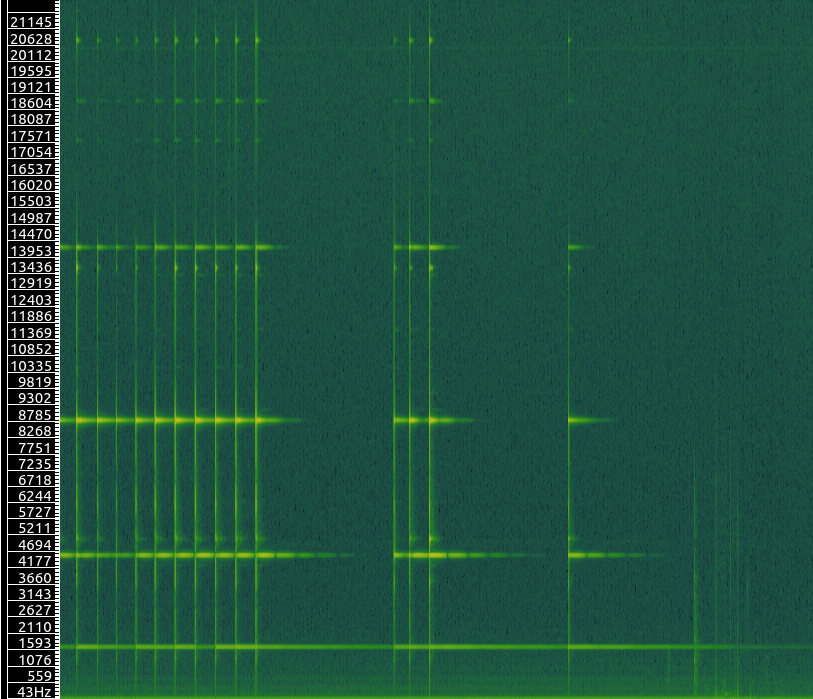
\includegraphics[width=0.65\textwidth]{prvni.png}
    \label{fig:uvod}
    \caption{Measurement for 15,3 cm long rod}
\end{figure}


\begin{figure}[H]
\centering
    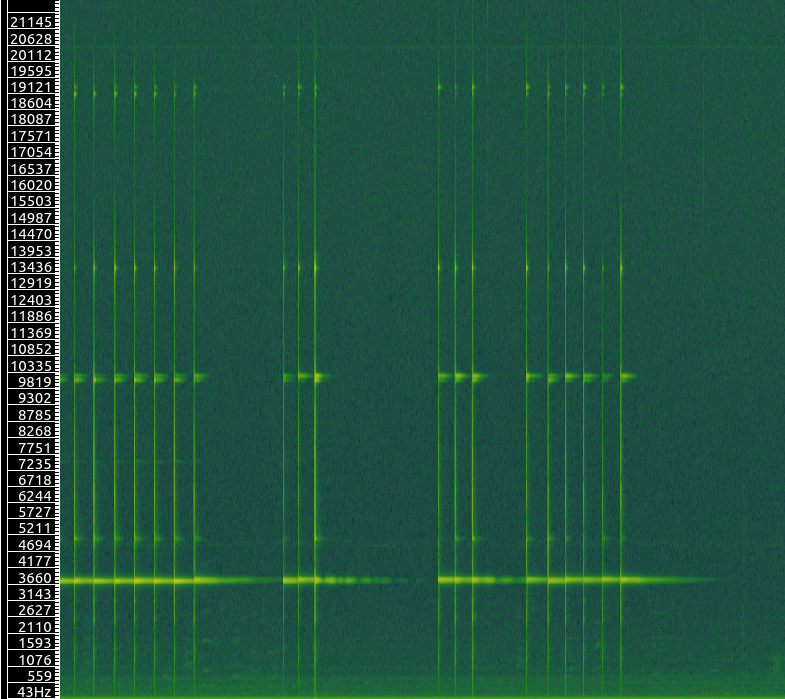
\includegraphics[width=0.65\textwidth]{druhy.png}
    \label{fig:uvod}
    \caption{Measurement for 10 cm long rod}
\end{figure}


\begin{figure}[H]
\centering
    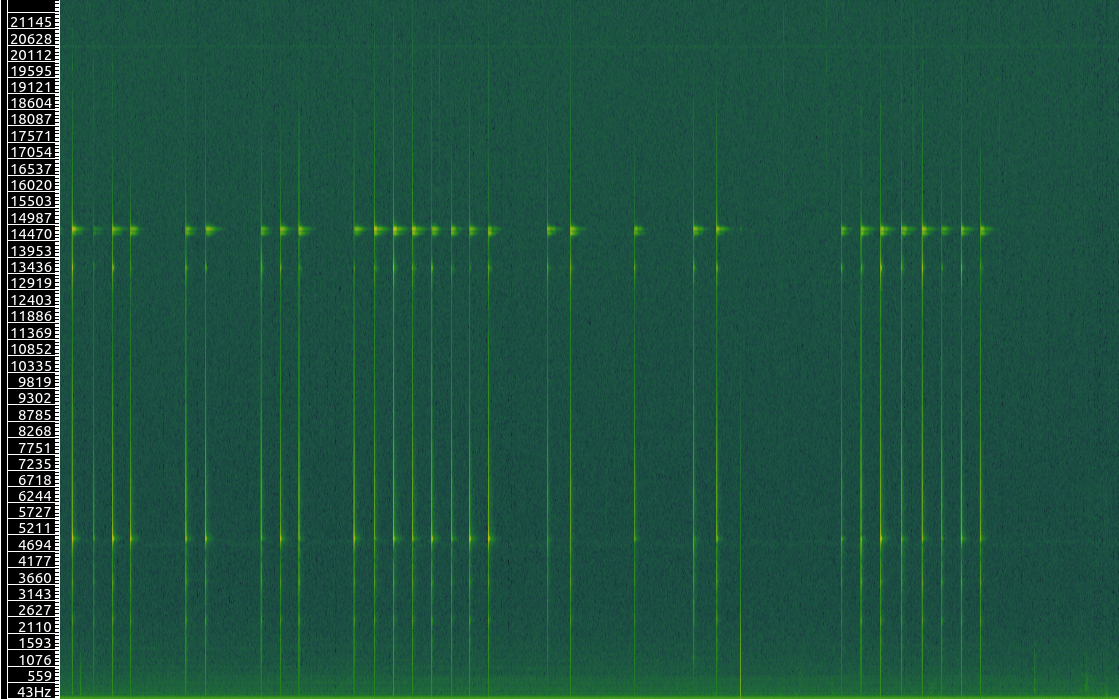
\includegraphics[width=0.65\textwidth]{treti.png}
    \label{fig:uvod}
    \caption{Measurement for 5 cm long rod}
\end{figure}

\newpage
\section{Final Discussion}
We would like to qualitatively explain the phenomenon: The changing magnetic field causes the material to change its shape. This effect is called magnetostriction and is being deeply studied in many works we found. We used one particular work we found. The geometry starts to be forced to change, which forces the rod to oscillate in the same direction as the change of the magnetic field. Then, due to inner asymmetry of ferrite rod oscillations transfer to other than longitudinal forms. The rod has its own natural frequencies and the intensity of the produced sound depends on the frequency of magnetic field. In fact, only frequencies very close to the natural ones make the rod produce hearable sound, as we found out during experiments. This time we mostly studied natural frequencies of the rod and the resonation, soon in future research we would like to study the way longitudinal waves transfer to bending waves, trying to predict which natural frequencies is ferrite rod more likely to oscillate on.
\section{Conclusion}
There are two main areas the problem includes: mechanical oscillations and magnetic properties of material. We tried to explain qualitatively, how oscillating magnetic field can cause oscillations in the rod. We as well tried to explain quantitatively which frequencies are capable of producing sound and our results were in good agreement with experiments.  We adumbrated how intensive sound produced by rod on each frequency can be. Now we are able to say what frequency is optimal, if we want the ferrite rod to produce sound.

\section{References}
\paragraph{}[1] IYPT 2020 Problems | IYPT.org. Official IYPT Website | IYPT.org [online]. Available from: \url{https://www.iypt.org/problems/problems-for-the-33rd-iypt-2020/}
\paragraph{}[2] Szewcyk, R.: Model of Magnetostrictive Hysteresis Loop with Local Maximum; Institute of Metrology and Biomedical Engineering, Warsaw University of Technology, 02-525 Warsaw, Poland
\paragraph{}[3] One-dimensional Elastodynamics, available from: \url{http://homepages.engineering.auckland.ac.nz/~pkel015/SolidMechanicsBooks/Part_II/02_1D_Elasticity/02_1D_Elasticity_02_Elastodynamics.pdf}
\paragraph{}[4] Parks, D. M.: Euler-Bernoulli Beams: Bending, Buckling and Vibration; Department of Mechanical Engineering MIT
\paragraph{}[5] Quality factor, available from: \url{https://www.electronics-notes.com/articles/basic_concepts/q-quality-factor/basics-tutorial-formula.php }

\newpage

\section{Appendix}
\subsection{First mechanical theory}
We can write down a Newton’s equation for every cut section on rod:
$$dm\frac{d^{2}y}{dt^{2}}+dF=0$$
We know, that each cut section oscillates around a point with potential minimum. For reason of conservation of energy we may say $$dF = dA \cdot y$$, for reason the movement to be harmonical. We continue.
$$dm\frac{d^{2}y}{dt^{2}}+ dA \cdot y=0$$
is a differential equation, his solution is $ sin(\omega \cdot t + \phi) $, where $ \omega $ is natural angular frequency of the oscillation and we can get it from our differential equation:
$$\omega=\sqrt{\frac{dA}{dm}}$$
From Euler-Bernoulli Beam theory we can get equation \footref{Euler}:
$$dA \cdot y =EI\cdot \frac{d^{4}y}{dx^{4}}dx$$
Due to harmonical movement we expect $y$ to be equal to $sin(\frac{2 \pi x}{\lambda})$, so fourth derivative would be $(\frac{2 \pi}{\lambda})^{4} \cdot sin(\frac{2 \pi x}{\lambda})$, so $dA=(\frac{2 \pi}{\lambda})^{4}EIdx$, $dm$ is, from definition, equal to $\rho \cdot S \cdot dx$, natural angular velocity will be equal to $ \sqrt{(\frac{2 \pi}{\lambda})^{4}\cdot \frac{EI}{\rho S}} $, so frequency will be: $$f = \frac{\omega}{2\pi} = \frac{2 \pi}{\lambda^{2}} \sqrt{\frac{E}{\rho}} \cdot \sqrt{\frac{I}{S}}$$
\subsection{Second mechanical theory}
In Appendix: First mechanical theory we expected the curve of the bended rod to be sinusoidal. We found out this is incorrect expectation. We used the same beginning equations but in Euler-Bernoulli Beam theory we said, $y$ is a periodical function with wavelength of $\lambda$. We can rewrite the function $y$ using Fourier series:
$$ y = \sum_{i}(a_{i} \cdot sin(\frac{2\pi xi}{\lambda}) + b_{i} \cdot cos(\frac{2\pi xi}{\lambda})) $$
And fourth derivative would be:
$$ \frac{d^{4}y}{dx^{4}} = \sum_{i}((\frac{2\pi xi}{\lambda})^{4} \cdot a_{i} \cdot sin(\frac{2\pi xi}{\lambda}) + (\frac{2\pi xi}{\lambda})^{4} \cdot b_{i} \cdot cos(\frac{2\pi xi}{\lambda})) = $$
$$
= (\frac{2\pi x}{\lambda})^{4} \cdot \sum_{i}(i^{4} \cdot a_{i} \cdot sin(\frac{2\pi xi}{\lambda}) + i^{4} \cdot b_{i} \cdot cos(\frac{2\pi xi}{\lambda})) = (\frac{2\pi x}{\lambda})^{4} \cdot p$$
We define a new function $p$, which has the same wavelength as $y$. So from Euler-Bernoulli Beam theory we get:
$$dA=(\frac{2\pi}{\lambda})^{4}4EI\cdot \frac{p}{q}$$
and from there and Newton's equation for rod cut section we get:
$$f=\frac{\omega}{2\pi}= \frac{2 \pi}{\lambda^{2}} \sqrt{\frac{E}{\rho}} \cdot \sqrt{\frac{I}{S}} \cdot \sqrt{\frac{p}{q}}$$
$\frac{p}{q}$ cannot depend on parameter $x$, as natural frequency cannot be different for different cut sections of the same rod, so we expect $\frac{p}{q}$ must be some sort of coefficient $k_{1}$, as well we expect, that wavelength is length of the rod multiplied by another coefficient $k_{2}$. From there we found expression:
$$f = \frac{k}{l^{2}} \cdot \sqrt{\frac{E}{\rho}} \cdot \sqrt{\frac{I}{S}}$$
\subsection{Processing data}
To find the change of amplitude of disrupted signal we developed our own method. At first, we used moving average technique to flatten the signal and free our function from some of disruptions. Then, for each measurement number n, we checked, if the value(n) is bigger than both value(n+1) and value(n-1). To this boolean we refer as to bool(n). Then, for each measurement number n, where bool(n) is equal to one, we check if value(n) is biggest of all values in nearby area, and if it is, we write down the measurement number as local maximum. From there we got the curve describing the amplitude of the disrupted signal.
\subsection{Finding Q factor}
In the circuit we have changing magnetic field. The energy stored in magnetic field is equal to $\frac{LI^{2}}{2}$, $I$ is equal to $GU$. Now we conclude, that $Q$ would be equal to $2\pi \frac{U_{n}^{2}}{U_{n}^{2} - U_{n + 1}^{2}}$. Due to the solution of differential equation of Inhibiting oscillator: $ a \frac{d^{2}y}{dx^{2}} + b \cdot \frac{dy}{dx} + c\cdot y = 0$, we expect the amplitude to descent exponentially. So we can write down equation $ U_{n+1}^{2} = \varrho \cdot U_n^{2}$, where $\varrho$ is a coefficient we can measure. If we want to measure amplitude difference between more than one wave we need to use another equation: $U_{n+m}^{2} = k ^{m} \cdot U_n^{2}$. From there we get $\sqrt[m]{\frac{U_{n+m}^{2}}{U_{n}^{2}}}$. Then $$ Q = 2\pi \frac{U_{n}^{2}}{\Delta \cdot U_{n}^{2}}  = 2\pi \frac{U_{n}^{2}}{U_{n}^{2} - k \cdot U_{n}^{2}} = \frac{2\pi}{1 - k} = \frac{2\pi}{1 - \sqrt[m]{\frac{U_{n + m}^{2}}{U_{n}^{2}}}}$$. Then we used technique described in Appendix: Processing data and experimentally found $U_{n}$, $U_{n+m}$ and $m$. From there we got $Q = 1,6103$.



\end{document}